\subsection{Dataset}
%%%%%%%%%%%%%%%%%%%%%%%%%%%%%%%%%%%%%%%%%%%%%%%%%%%%%
In this work, we have generated a large dataset of 475 cases of a full wavefield of propagating Lamb waves in a plate made of carbon fibre-reinforced plastic (CFRP).
The in-house code of the time-domain spectral element method was used for simulation of Lamb wave interaction with delamination~\cite{Kudela2020}.
It should be added that despite the utilisation of the parallel code of the spectral element method which was run on the Tesla K20X GPU card, the computation of the dataset (consisting of 475 cases) took about 3 months.
For each case, single delamination was modelled by using the method of splitting nodes between appropriate spectral elements. 
It was assumed that the composite laminate is made of eight layers of a total thickness of 3.9 mm.
The delamination was modelled between the third and fourth layer (see Fig.~\ref{fig:plate_setup} for details).
It should be noted that Fig.~\ref{fig:plate_setup} shows an exaggerated cross-section through the delamination. 
Zero-volume delamination was assumed in the model. 
Delamination spatial location was selected randomly so that the interaction of guided waves with delamination is different for each case.
It includes cases when delamination is located at the edge of the plate which is the most difficult to identify by signal processing methods.
Additionally, the size of the delamination of elliptic shape was randomly simulated by selecting the size of ellipse minor and major axis.
Also, the angle between the delamination major axis and the horizontal axis was randomly selected.
In summary the following random factors were simulated in each case:
\begin{itemize}
\item delamination geometrical size	(ellipse minor and major axis randomly selected from the interval \(\left[10 \, \textrm{mm}, 40\, \textrm{mm}\right]\)),
\item delamination angle (randomly selected from the interval \( \left[ 0^{\circ}, 180^{\circ} \right]\)),
\item coordinates of the centre of delamination (randomly selected from the interval \(\left[0\, \textrm{mm}, 250\, \textrm{mm} -\delta \right]\) and \( \left[250\, \textrm{mm}+\delta, 500\, \textrm{mm} \right] \), where \(\delta = 10\, \textrm{mm}\)).
\end{itemize}
It resulted in random spatial placement of delaminations. The plate with overlayed 475 delamination cases is shown in Fig.~\ref{fig:random_delam}.
\begin{figure}
	\centering
	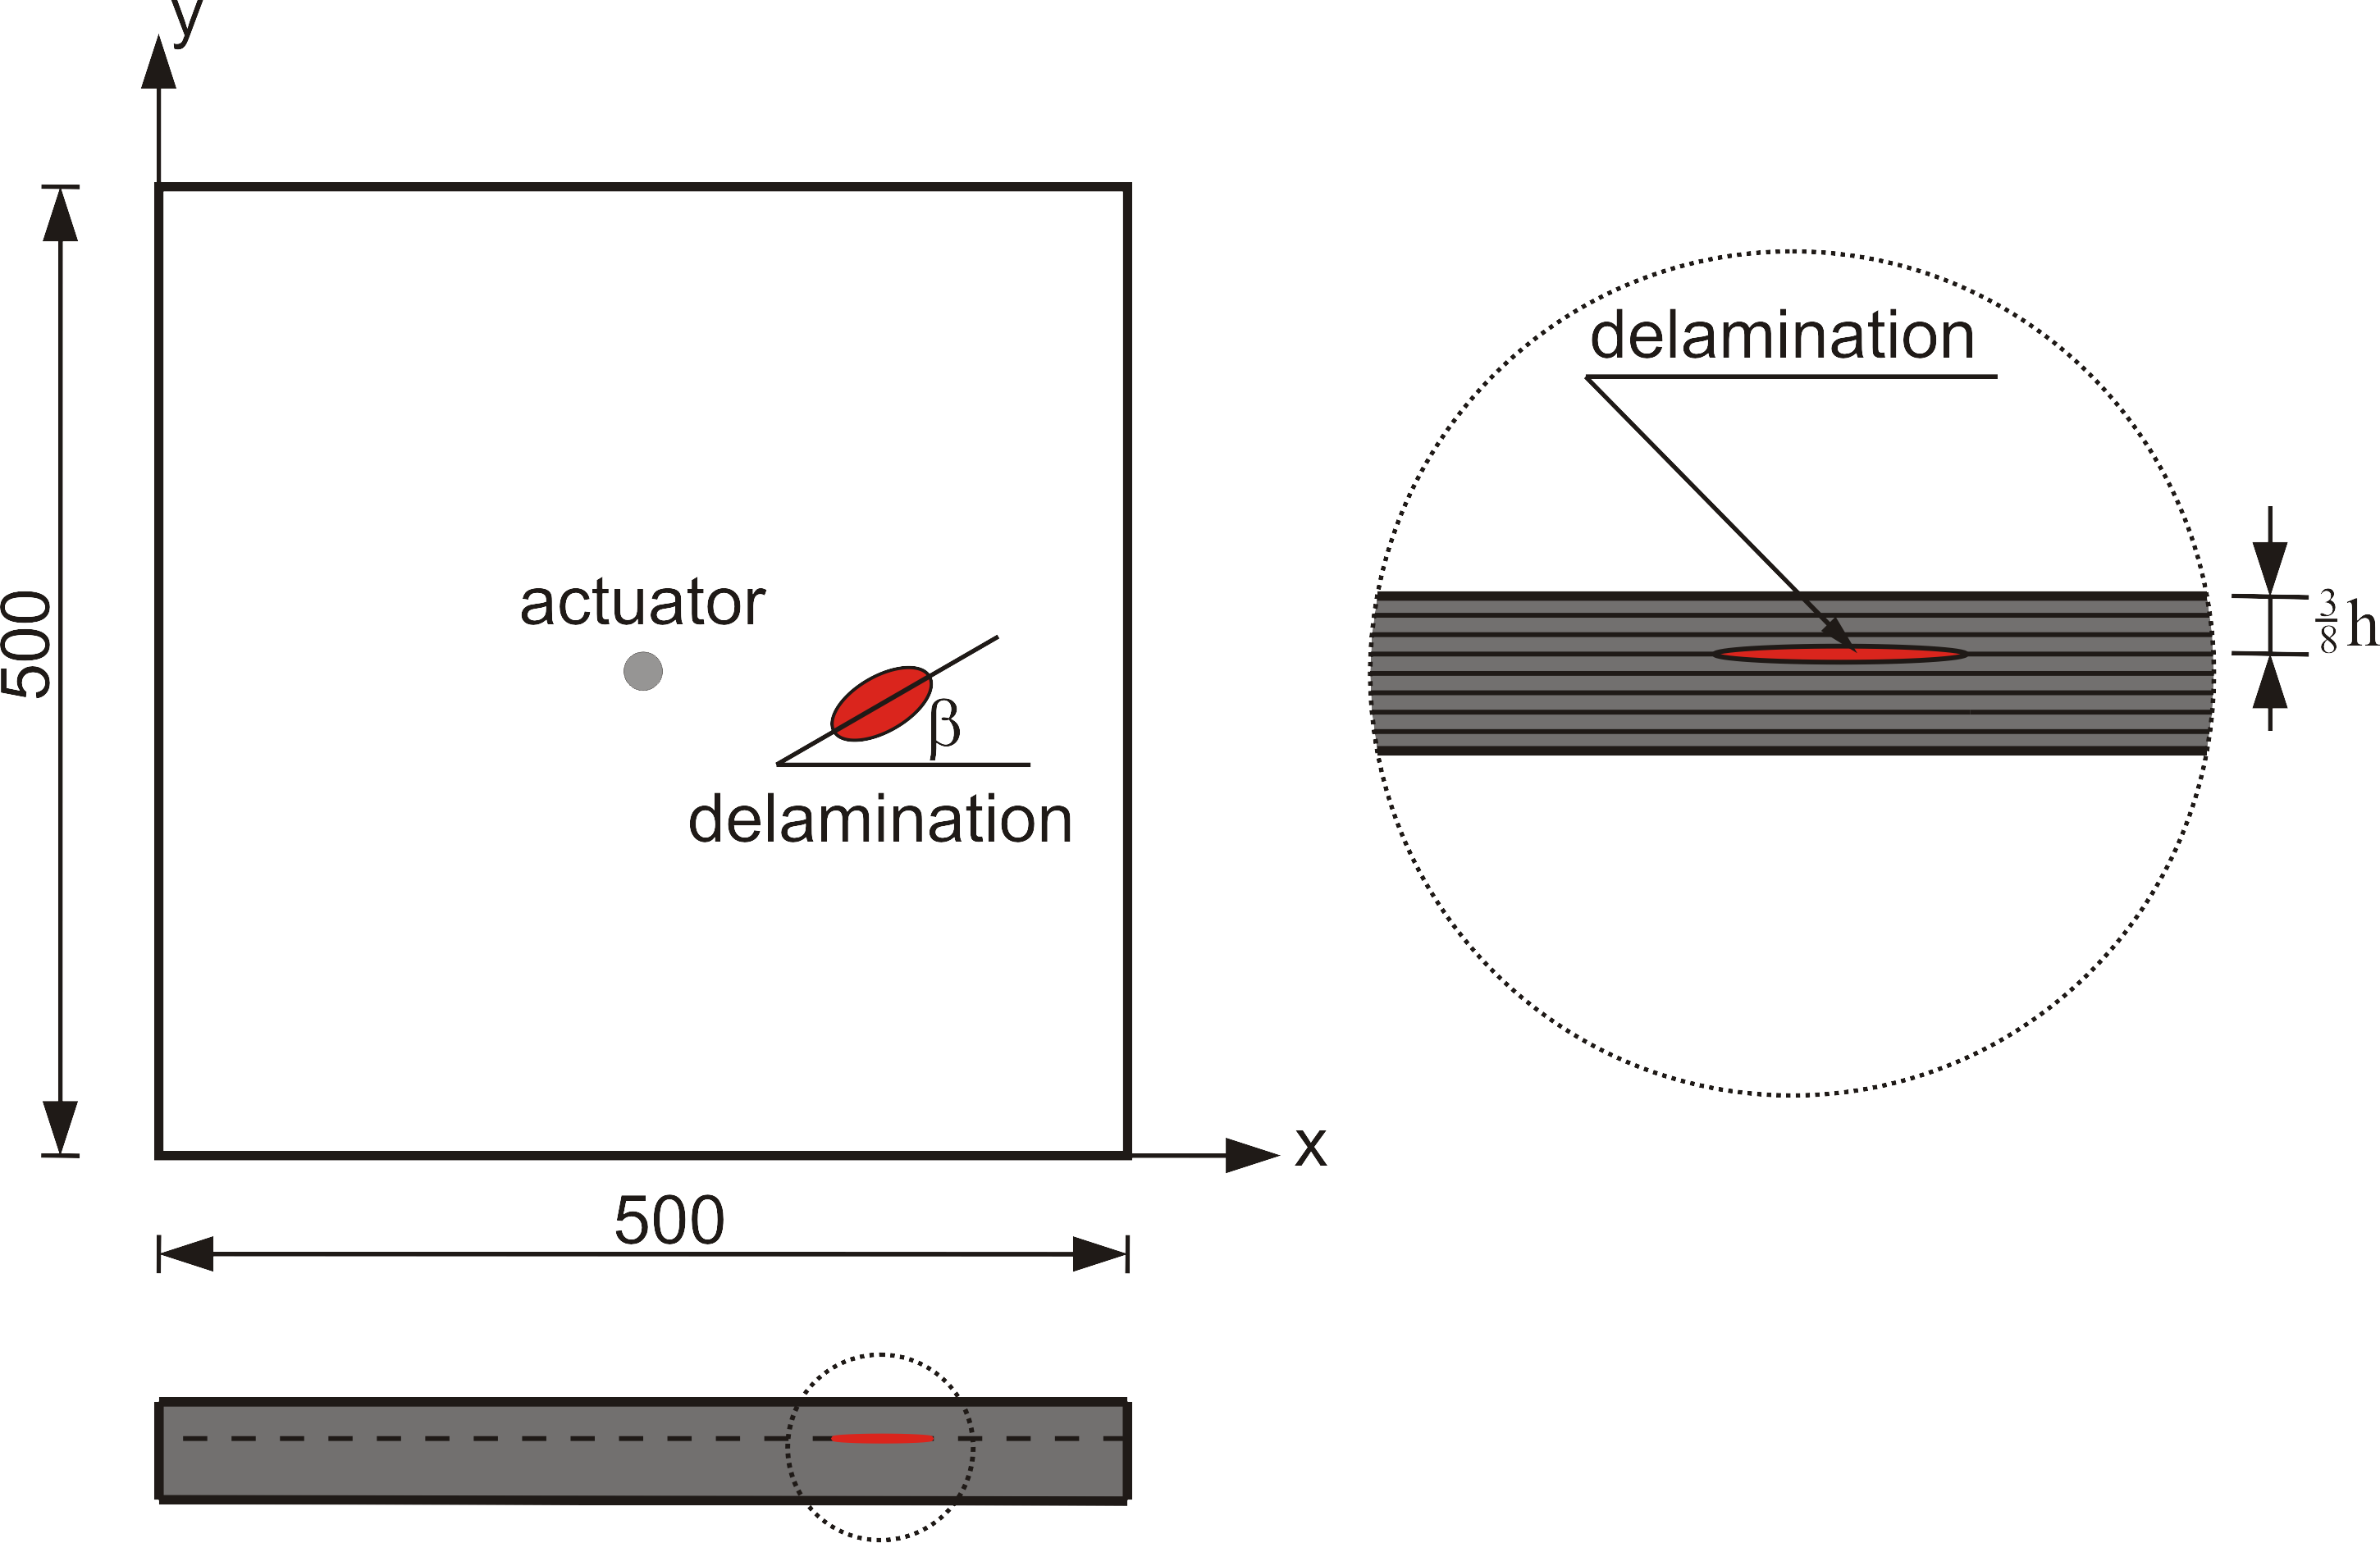
\includegraphics[scale=0.8]{plate_delam_arrangement_MSSP.png}
	\caption{Setup for computing Lamb wave interactions with delamination.}
	\label{fig:plate_setup}
\end{figure}	
\begin{figure}
	\centering
	\includegraphics[scale=1]{dataset2_labels_ellipses.png}
	\caption{The plate with 475 cases of random delaminations.}
	\label{fig:random_delam}
\end{figure}
		
Guided waves were excited at the plate centre by applying equivalent piezoelectric forces.
The excitation signal had a form of sinusoid modulated by Hann window. 
It was assumed that the carrier frequency is 50 kHz and the modulation frequency is 10 kHz.
A relatively low carrier frequency allowed for lower mesh density and significant computation time reduction in comparison to simulations of higher frequencies.
Additionally, the excitation signal was selected so that interaction of generated A0 Lamb wave mode with the smallest delamination can be still used as a feature for damage identification.

The output from the top and bottom surfaces of the plate in the form of particle velocities at the nodes of spectral elements were interpolated on the uniform grid of 500\(\times\)500 points by using shape functions of elements (see~\cite{Kudela2020} for more details).
It essentially resembles measurements acquired by SLDV in the transverse direction (perpendicular to the plate surface).
An example of the simulated full wavefield data on the top and bottom surfaces is presented in Fig.~\ref{fig:wavefield}.
It should be noted that stronger wave entrapment at delamination can be observed for the case of the wavefield at the top surface.
It is because the delamination within cross-section is located closer to the top surface.
It makes it easier to detect delamination by processing wavefield at the top surface.
It is better visible if the root mean square (RMS) according to Eq.~(\ref{eq:rms}) is applied to the wavefield.
The result of this operation is presented in Fig.~\ref{fig:rms}.
Based on the image analysis, the shape of the delamination can be easier to discern for the top case.
However, the methodology presented in this paper was applied to the more difficult case i.e. wavefield registered at the bottom surface of the plate.

The dataset consisting of RMS images which were used in this research paper is available online~\cite{Kudela2020d}.

\begin{figure} [h!]
	\centering
	\begin{subfigure}[b]{0.32\textwidth}
		\centering
		\includegraphics[scale=1]{96_flat_shell_Vz_1_500x500top.png}
		\caption{\(t=0.141\) ms}
		\label{fig:frame96top}
	\end{subfigure}
	\hfill
	\begin{subfigure}[b]{0.32\textwidth}
		\centering
		\includegraphics[scale=1]{128_flat_shell_Vz_1_500x500top.png}
		\caption{\(t=0.188\) ms}
		\label{fig:frame128top}
	\end{subfigure}
	\hfill
	\begin{subfigure}[b]{0.32\textwidth}
		\centering
		\includegraphics[scale=1]{164_flat_shell_Vz_1_500x500top.png}
		\caption{\(t=0.240\) ms}
		\label{fig:frame164top}
	\end{subfigure}	
	\hfill
	\begin{subfigure}[b]{0.32\textwidth}
		\centering
		\includegraphics[scale=1]{96_flat_shell_Vz_1_500x500bottom.png}
		\caption{\(t=0.141\) ms}
		\label{fig:frame96bottom}
	\end{subfigure}
	\hfill
	\begin{subfigure}[b]{0.32\textwidth}
		\centering
		\includegraphics[scale=1]{128_flat_shell_Vz_1_500x500bottom.png}
		\caption{\(t=0.188\) ms}
		\label{fig:frame128bottom}
	\end{subfigure}
	\hfill
	\begin{subfigure}[b]{0.32\textwidth}
		\centering
		\includegraphics[scale=1]{164_flat_shell_Vz_1_500x500bottom.png}
		\caption{\(t=0.240\) ms}
		\label{fig:frame164bottom}
	\end{subfigure}

	\caption{Full wavefield at the top surface (a)--(c) and the bottom surface (d)--(f), respectively, at selected time instances showing the interaction of guided waves with delamination.}
	\label{fig:wavefield}
\end{figure} 

\begin{figure} [h!]
	\centering
	\begin{subfigure}[b]{0.47\textwidth}
		\centering
		\includegraphics[scale=1]{RMS_flat_shell_Vz_1_500x500top.png}
		\caption{top}
		\label{fig:rmstop}
	\end{subfigure}
	\hfill
	\begin{subfigure}[b]{0.47\textwidth}
		\centering
		\includegraphics[scale=1]{RMS_flat_shell_Vz_1_500x500bottom.png}
		\caption{bottom}
		\label{fig:rmsbottom}
	\end{subfigure}
	\caption{RMS of the full wavefield from the top surface of the plate (a) and the bottom surface of the plate (b).}
\label{fig:rms}
\end{figure} 